\subsection{Valg af systemdefinition}
\label{subsec:valgafsystemdefinition}

%SYSTEMVALG
Vi holdte os meget åbne for nye løsningsforslag, da vi gerne ville gøre det muligt for informanterne at komme med nye idéer, også selvom de var markant anderledes end vores systemdefinitioner. Vi ønskede at høre om informanterne ville være i stand til bruge lignende systemer. Derfor foregik møderne som semistrukturerede interviews, hvilket betyder, at vi havde udformet et interview med spørgsmål, som vi ønskede at stille, men der var luft i interviewet til at informanterne kunne introducere nye emner til diskussionen. Disse nye emner ville ikke ødelægge interviewet. Det var vigtigt for os at få informanternes idéer til hvilke funktioner et sådan system skulle have, og hvilke krav de stiller. 

Der blev taget højde for informanternes respons (Al dokumentation og alle referater fra de afholdte møder med informanterne kan findes i \apref{ap:informant}.) på de udarbejdede systemdefinitioner, og der blev truffet et valg, som alle parter kan se som en mulig løsning på problemerne mht. madlavning og madspild i danske husstande. Efter møderne var det helt klart, hvilken systemdefinition, der var den, informanterne ønskede. Med hensyn til systemdefinition 2 (se \secref{subsec:alternativesystemdefinitioner}) mente informanterne, at de simpelthen ikke ville komme til at bruge et planlægningsværktøj, da det ville være både for tidskrævende og give dem mindre frihed. Systemdefinition 1 (se \secref{subsec:alternativesystemdefinitioner}) var informanterne derimod meget entusiastiske overfor. De så systemdefinition 1 som et meget brugbart system, der ville gøre det muligt for dem at bruge deres gamle madrester på en spændende måde. På baggrund af dette valgte vi at udvikle systemet som beskrevet i \textbf{systemdefinition 1}. Denne beslutning satte nogle fastere rammer for projektets videre forløb. En visualisering af systemet kan ses i \figref{fig:rigbillede2}.

\begin{figure}
	\centering
	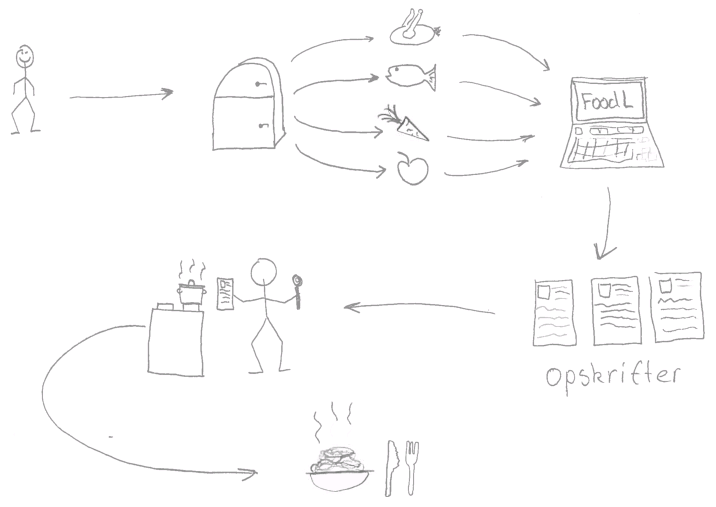
\includegraphics[scale=0.6]{billeder/rigebilleder/anvendelsesomraade.png}
	\capt{Rigt billede, der visualiserer anvendelsen af systemet udtrykt i systemdefinition 1.}
	\label{fig:rigbillede2}
\end{figure}

%AFSLUTNING
Systemdefinition 1 er blevet valgt. Det er nu på tide at overveje, hvordan systemet skal fungere, hvordan det skal designes, og hvilke funktioner, der skal inkluderes i systemet.
